\section{Numerical Experiments}


\subsection{Polarization}

The goal of the numerical experiments presented in this section is investigating the opinion polarization within a population using our model. In particular, we aim to understand how the model parameters influence the polarization. 
Polarization refers either to a distribution of opinions with multiple local maxima or to the process by which such strong divergences of opinions that divide a population come about \cite{Banisch2019}\cite{Bramsona2016}. The model presented in Section~\ref{sec:mathematical} has been slightly modified for what concerns the link weights. If $s_i$ denotes the similarity of individual $i$, then the entry $a_{ij} = a_{ji}$ is 
\begin{equation}
a_{ij} = \text{max}\{0, \delta_{ij} + 0.2\ r\}
\end{equation}
where $r$ is a random number from normal distribution $\mathcal{N}(0,1)$ and $\delta_{ij} = 1$ if $s_i = s_j$ otherwise $\delta_{ij} = 0$. 

The number of real and fake sources is 3. Influencability and critical thinking traits are set to $0.5$ for all individuals. Similarity is set to $1$ for half of individuals and to $0$ for the second half. Thus, the probability of creating a link remains the same, but the weight of the link has is around 1 if the node belong to the same half and non-negative and close to 0 if they belong to different halves. An example of a single experiment is shown in Figure~\ref{pics:exp20}.\\

\begin{figure}[!t]
\centering
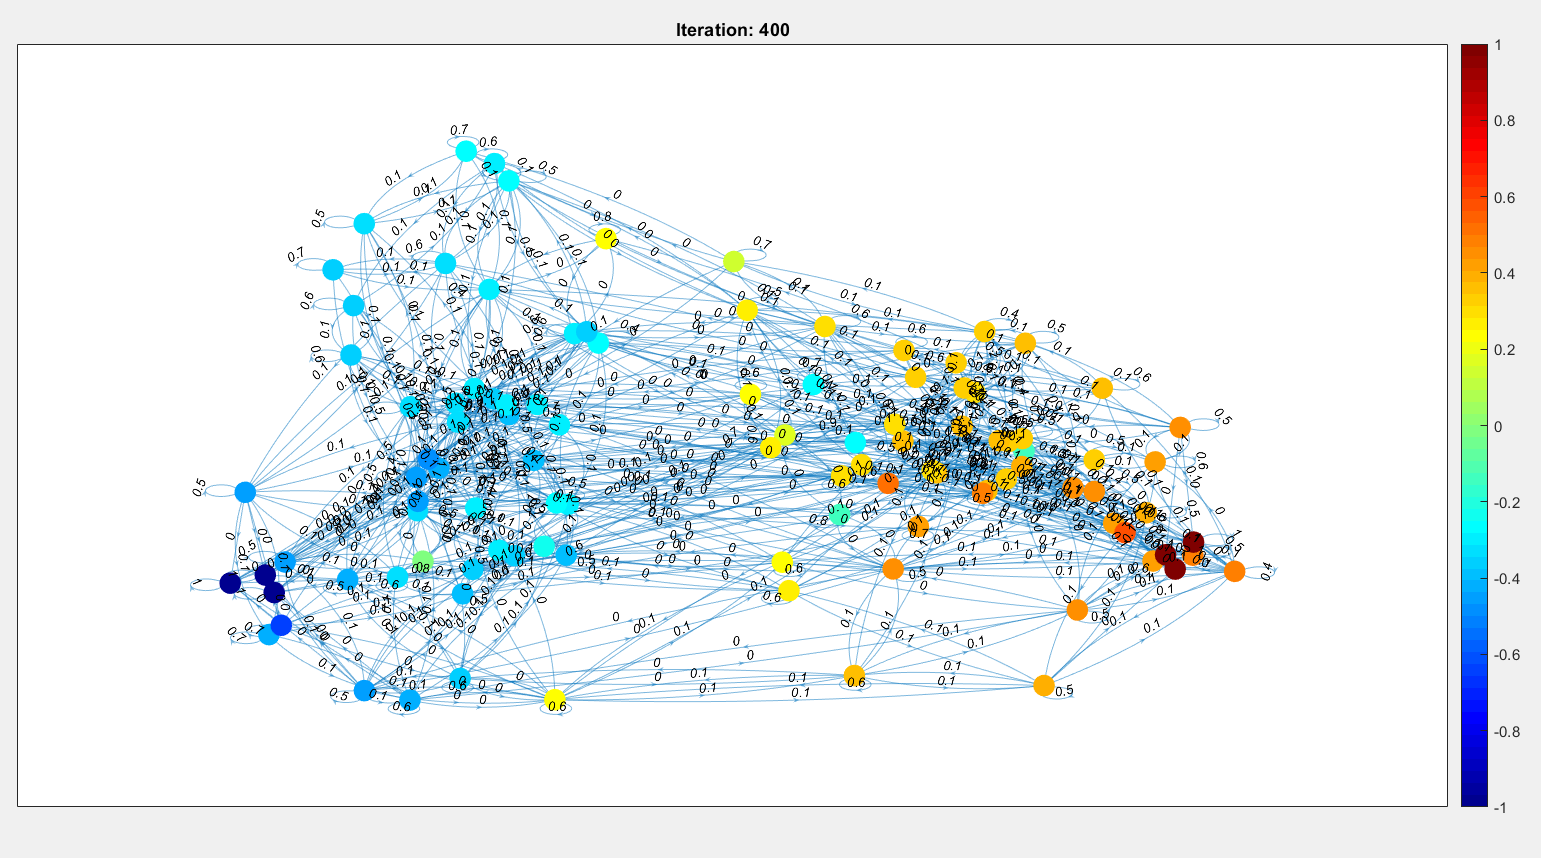
\includegraphics[width=8cm]{Figures/Exp20_graph.png}
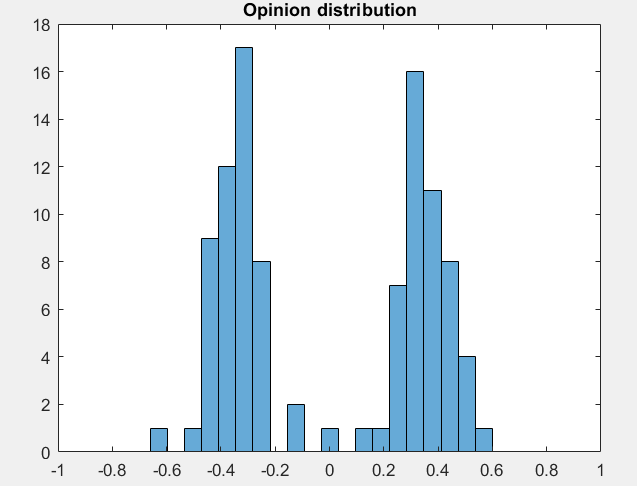
\includegraphics[width=8cm]{Figures/Exp20_hyst.png}
\caption{Simulation with 100 individuals, 3 sources of Fake and 3 of Real News, $C=0.2$, nRoot$=4$ and new connection local. Above: graph at steady state. Below: opinion distribution at steady sate.}
\label{pics:exp20}
\end{figure}

To the best of our knowledge, there is not a unique metric to quantify opinion polarization. We used the measure proposed in \cite{Matakos2017} defined as $R_2 = ||x_{\infty}||^2/ N$, the standard deviation of $x_{\infty}$ according to the interpretation of polarization as dispersion exposed in \cite{Bramsona2016} and the mean.\\

In our experiments, we varied three parameters: $C$ in the range $[0.2; 0.6]$, nRoot in the range $[2; 8]$ and the news connection, which is either local or spread. For each parameters combination, 100 cases have been randomly generated and the average metrics have been computed for the opinion vector at steady state.\\

The mean is at  $0 \pm 5\times 10^{-3}$ for all cases, which means that there is not a predominant opinion. This is expected, because the parametrization does not favour one opinion. When the news sources are spread, the average is even closer to 0 ($0 \pm 10^{-3}$). Although in this section we are not interested in the average opinion, the fact that the mean is close to 0 makes the standard deviation and $R_2$ good metrics to evaluate the polarization. A high standard deviation correspond to many entries far from the center on both sides of the opinion spectrum.\\

Because of the mean $\overline{x}$ close to 0 and $N=100$, we have
$$ \sigma^2 = \frac{1}{N} \sum_{i=1}^N x_i (x_i-\overline{x})^2 \approx \frac{1}{N} \sum_{i=1}^N x_i^2 = R_2.$$

Thus, the two metrics carry the same information about the polarization and, for sake of simplicity, we only discuss the standard deviation. Results for 30 parameters combinations are shown in Figure~\ref{pics:pol_std}. Since the opinions are between $-1$ and $1$, the standard deviation is between 0 and 1.\\

We notice that the higher $C$ and nRoot are, the less polarized are the opinions. Moreover, the higher lower nRoot is, the faster grows the polarization by decreasing $C$. This is in line with our expectations. The higher is $C$, the more likely contacts are and is proportional to the average in and out degree of each node. A high nRoot means that each individual is more likely to have a link with another individual which is far and, in this case, contacts among individuals with different similarity are more likely. Thus, the experiments show that polarization arises in the society when individuals are in contact with few other people or when they are in contact mainly with similar people. The strongest polarization is present when both conditions are met.\\

Another remarkable result is the comparison between the cases where the news are local (blue) and when they are spread (red). Spreading the news reduces the polarization in the network. 
For each $C$ and nRoot combination, the standard deviation is at most one third of the value for the corresponding case with local news. Also with spread news we observe an increase of polarization when $C$ and nRoot decrease, but the growth is less strong. This experiment suggest that a society where each individual has the chance to come in touch with all news sources and not only the ones close to their milieu, is less likely be polarized.
\acomment{riferimento a letteratura? evitare di dare troppo significato!}

\begin{figure}[!t]
\centering
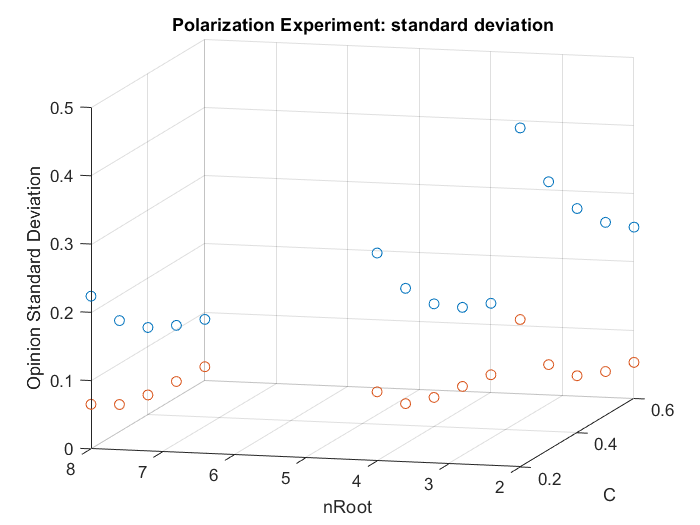
\includegraphics[width=8cm]{Figures/pol_std1.png}
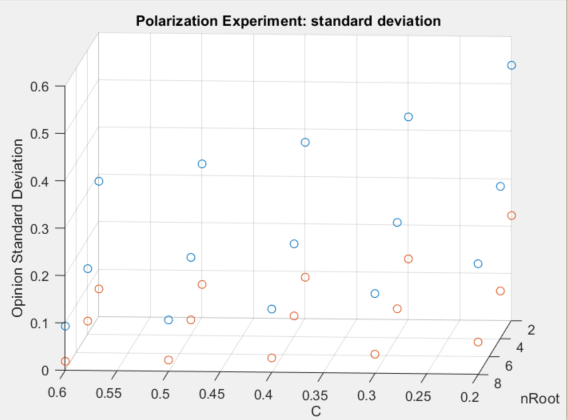
\includegraphics[width=8cm]{Figures/pol_std2.png}
\caption{Standard deviation for different combinations of C, nRoot and news connection. Red: news are spread. Blue: news are local.}
\label{pics:pol_std}
\end{figure}










